% Options for packages loaded elsewhere
\PassOptionsToPackage{unicode}{hyperref}
\PassOptionsToPackage{hyphens}{url}
%
\documentclass[
]{book}
\usepackage{amsmath,amssymb}
\usepackage{lmodern}
\usepackage{iftex}
\ifPDFTeX
  \usepackage[T1]{fontenc}
  \usepackage[utf8]{inputenc}
  \usepackage{textcomp} % provide euro and other symbols
\else % if luatex or xetex
  \usepackage{unicode-math}
  \defaultfontfeatures{Scale=MatchLowercase}
  \defaultfontfeatures[\rmfamily]{Ligatures=TeX,Scale=1}
\fi
% Use upquote if available, for straight quotes in verbatim environments
\IfFileExists{upquote.sty}{\usepackage{upquote}}{}
\IfFileExists{microtype.sty}{% use microtype if available
  \usepackage[]{microtype}
  \UseMicrotypeSet[protrusion]{basicmath} % disable protrusion for tt fonts
}{}
\makeatletter
\@ifundefined{KOMAClassName}{% if non-KOMA class
  \IfFileExists{parskip.sty}{%
    \usepackage{parskip}
  }{% else
    \setlength{\parindent}{0pt}
    \setlength{\parskip}{6pt plus 2pt minus 1pt}}
}{% if KOMA class
  \KOMAoptions{parskip=half}}
\makeatother
\usepackage{xcolor}
\usepackage{color}
\usepackage{fancyvrb}
\newcommand{\VerbBar}{|}
\newcommand{\VERB}{\Verb[commandchars=\\\{\}]}
\DefineVerbatimEnvironment{Highlighting}{Verbatim}{commandchars=\\\{\}}
% Add ',fontsize=\small' for more characters per line
\usepackage{framed}
\definecolor{shadecolor}{RGB}{248,248,248}
\newenvironment{Shaded}{\begin{snugshade}}{\end{snugshade}}
\newcommand{\AlertTok}[1]{\textcolor[rgb]{0.94,0.16,0.16}{#1}}
\newcommand{\AnnotationTok}[1]{\textcolor[rgb]{0.56,0.35,0.01}{\textbf{\textit{#1}}}}
\newcommand{\AttributeTok}[1]{\textcolor[rgb]{0.77,0.63,0.00}{#1}}
\newcommand{\BaseNTok}[1]{\textcolor[rgb]{0.00,0.00,0.81}{#1}}
\newcommand{\BuiltInTok}[1]{#1}
\newcommand{\CharTok}[1]{\textcolor[rgb]{0.31,0.60,0.02}{#1}}
\newcommand{\CommentTok}[1]{\textcolor[rgb]{0.56,0.35,0.01}{\textit{#1}}}
\newcommand{\CommentVarTok}[1]{\textcolor[rgb]{0.56,0.35,0.01}{\textbf{\textit{#1}}}}
\newcommand{\ConstantTok}[1]{\textcolor[rgb]{0.00,0.00,0.00}{#1}}
\newcommand{\ControlFlowTok}[1]{\textcolor[rgb]{0.13,0.29,0.53}{\textbf{#1}}}
\newcommand{\DataTypeTok}[1]{\textcolor[rgb]{0.13,0.29,0.53}{#1}}
\newcommand{\DecValTok}[1]{\textcolor[rgb]{0.00,0.00,0.81}{#1}}
\newcommand{\DocumentationTok}[1]{\textcolor[rgb]{0.56,0.35,0.01}{\textbf{\textit{#1}}}}
\newcommand{\ErrorTok}[1]{\textcolor[rgb]{0.64,0.00,0.00}{\textbf{#1}}}
\newcommand{\ExtensionTok}[1]{#1}
\newcommand{\FloatTok}[1]{\textcolor[rgb]{0.00,0.00,0.81}{#1}}
\newcommand{\FunctionTok}[1]{\textcolor[rgb]{0.00,0.00,0.00}{#1}}
\newcommand{\ImportTok}[1]{#1}
\newcommand{\InformationTok}[1]{\textcolor[rgb]{0.56,0.35,0.01}{\textbf{\textit{#1}}}}
\newcommand{\KeywordTok}[1]{\textcolor[rgb]{0.13,0.29,0.53}{\textbf{#1}}}
\newcommand{\NormalTok}[1]{#1}
\newcommand{\OperatorTok}[1]{\textcolor[rgb]{0.81,0.36,0.00}{\textbf{#1}}}
\newcommand{\OtherTok}[1]{\textcolor[rgb]{0.56,0.35,0.01}{#1}}
\newcommand{\PreprocessorTok}[1]{\textcolor[rgb]{0.56,0.35,0.01}{\textit{#1}}}
\newcommand{\RegionMarkerTok}[1]{#1}
\newcommand{\SpecialCharTok}[1]{\textcolor[rgb]{0.00,0.00,0.00}{#1}}
\newcommand{\SpecialStringTok}[1]{\textcolor[rgb]{0.31,0.60,0.02}{#1}}
\newcommand{\StringTok}[1]{\textcolor[rgb]{0.31,0.60,0.02}{#1}}
\newcommand{\VariableTok}[1]{\textcolor[rgb]{0.00,0.00,0.00}{#1}}
\newcommand{\VerbatimStringTok}[1]{\textcolor[rgb]{0.31,0.60,0.02}{#1}}
\newcommand{\WarningTok}[1]{\textcolor[rgb]{0.56,0.35,0.01}{\textbf{\textit{#1}}}}
\usepackage{longtable,booktabs,array}
\usepackage{calc} % for calculating minipage widths
% Correct order of tables after \paragraph or \subparagraph
\usepackage{etoolbox}
\makeatletter
\patchcmd\longtable{\par}{\if@noskipsec\mbox{}\fi\par}{}{}
\makeatother
% Allow footnotes in longtable head/foot
\IfFileExists{footnotehyper.sty}{\usepackage{footnotehyper}}{\usepackage{footnote}}
\makesavenoteenv{longtable}
\usepackage{graphicx}
\makeatletter
\def\maxwidth{\ifdim\Gin@nat@width>\linewidth\linewidth\else\Gin@nat@width\fi}
\def\maxheight{\ifdim\Gin@nat@height>\textheight\textheight\else\Gin@nat@height\fi}
\makeatother
% Scale images if necessary, so that they will not overflow the page
% margins by default, and it is still possible to overwrite the defaults
% using explicit options in \includegraphics[width, height, ...]{}
\setkeys{Gin}{width=\maxwidth,height=\maxheight,keepaspectratio}
% Set default figure placement to htbp
\makeatletter
\def\fps@figure{htbp}
\makeatother
\setlength{\emergencystretch}{3em} % prevent overfull lines
\providecommand{\tightlist}{%
  \setlength{\itemsep}{0pt}\setlength{\parskip}{0pt}}
\setcounter{secnumdepth}{5}
\usepackage{booktabs}
\ifLuaTeX
  \usepackage{selnolig}  % disable illegal ligatures
\fi
\usepackage[]{natbib}
\bibliographystyle{apalike}
\IfFileExists{bookmark.sty}{\usepackage{bookmark}}{\usepackage{hyperref}}
\IfFileExists{xurl.sty}{\usepackage{xurl}}{} % add URL line breaks if available
\urlstyle{same} % disable monospaced font for URLs
\hypersetup{
  pdftitle={Bayesian Inference and Computation},
  pdfauthor={Dr Rowland Seymour},
  hidelinks,
  pdfcreator={LaTeX via pandoc}}

\title{Bayesian Inference and Computation}
\author{Dr Rowland Seymour}
\date{Semester 2, 2023}

\usepackage{amsthm}
\newtheorem{theorem}{Theorem}[chapter]
\newtheorem{lemma}{Lemma}[chapter]
\newtheorem{corollary}{Corollary}[chapter]
\newtheorem{proposition}{Proposition}[chapter]
\newtheorem{conjecture}{Conjecture}[chapter]
\theoremstyle{definition}
\newtheorem{definition}{Definition}[chapter]
\theoremstyle{definition}
\newtheorem{example}{Example}[chapter]
\theoremstyle{definition}
\newtheorem{exercise}{Exercise}[chapter]
\theoremstyle{definition}
\newtheorem{hypothesis}{Hypothesis}[chapter]
\theoremstyle{remark}
\newtheorem*{remark}{Remark}
\newtheorem*{solution}{Solution}
\begin{document}
\maketitle

{
\setcounter{tocdepth}{1}
\tableofcontents
}
\hypertarget{practicalities}{%
\chapter*{Practicalities}\label{practicalities}}
\addcontentsline{toc}{chapter}{Practicalities}

\hypertarget{module-aims}{%
\section{Module aims}\label{module-aims}}

The module aims to give you an overview of the Bayesian paradigm. By the end of the course, you should

\begin{enumerate}
\def\labelenumi{\arabic{enumi}.}
\item
  Be able to conceptualise a Bayesian approach for statistics
\item
  Be able to derive posterior and posterior predictive distributions for uni- and multivariate models
\item
  Identify suitable prior distributions and understand how the choice of prior distribution may affect the final result
\item
  Understand the principles of Markov Chain Monte Carlo and be able to construct an MCMC algorithm
\end{enumerate}

\hypertarget{module-structure}{%
\section{Module structure}\label{module-structure}}

The module is split between theory and programming. Each week (excluding week 6) will have two lectures and two computer labs.

\hypertarget{assessment}{%
\section{Assessment}\label{assessment}}

The module is 55\% coursework and 45\% exam. The exam will last 1h 30m and take place during the summer exam period. More details about the coursework will be announced during the semester.

\hypertarget{getting-help}{%
\section{Getting help}\label{getting-help}}

There are lots of ways of getting help throughout the module. You can visit my office hour (Watson 317) on \ldots.. or email me at \href{mailto:r.g.seymour@bham.ac.uk}{\nolinkurl{r.g.seymour@bham.ac.uk}}. Each week, there will also be a problem class.

\hypertarget{recommended-books-and-videos}{%
\section{Recommended books and videos}\label{recommended-books-and-videos}}

No books are required for this course and the whole material is contained in these notes. However, you may find it useful to use other resources in your studies. I recommend the following:

\begin{enumerate}
\def\labelenumi{\arabic{enumi}.}
\item
  \href{https://link.springer.com/book/10.1007/978-0-387-92407-6}{A First Course in Bayesian Statistical Methods - Peter D. Hoff}. This is a short book that covers the basics of Bayesian inference and computation. To the point and well written, it's a useful place to look topics up.
\item
  \href{http://www.stat.columbia.edu/~gelman/book/}{Bayesian Data Analysis - Andrew Gelman, John Carlin, Hal Stern, David Dunson, Aki Vehtari, and Donald Rubin}. This is a thorough book explaining everything you'd need to know to carry out Bayesian data analysis. It's a fairly look and in-depth book, but the authors are authoritative and give good advice throughout. Example code on the website is in R, Python and Stan.
\item
  \href{https://xcelab.net/rm/statistical-rethinking/}{Statistical Rethinking - Richard McElrath}. This book provides a friendly intuitive understanding of Bayesian inference and computation. Aimed at social and natural scientists, it has less theory that the other two books but is perhaps more approachable. A set of video lectures for this book can be found \href{https://www.youtube.com/playlist?list=PLDcUM9US4XdMROZ57-OIRtIK0aOynbgZN}{on YouTube}.
\end{enumerate}

\hypertarget{fundamentals}{%
\chapter{Fundamentals of Bayesian inference}\label{fundamentals}}

Bayesian inference is built on a different way of thinking about probability that methods you have learnt so far. In the past 30 years or so, Bayesian inference has become much more popular. This is partly due to increased computational power becoming available. In this first chapter, we are going to set out:

\begin{enumerate}
\def\labelenumi{\arabic{enumi}.}
\item
  What are the fundamental principles of Bayesian inference?
\item
  What makes Bayesian inference different from other methods?
\end{enumerate}

\hypertarget{statistical-inference}{%
\section{Statistical Inference}\label{statistical-inference}}

Three purpose of statistical inference is to ``draw conclusions, from numerical data, about quantities that are not observed'' (Bayesian Data Analysis, chapter 1). Generally speaking there are two kinds of inference: inference for quantities that are not possible to observe, and inference for quantities that unobserved or hasn't happened yet. We can apply our inference methods to a huge range of applications, from the effectiveness of drugs in a clinical trial, to estimating the number of victims of violence against women and girls.

In this module, we are going to look at a different way of carrying out statistical inference, one that doesn't depend on long running event. Instead, we're going to introduce the definition of probability that allows us to Interpret the subjective chance that an event occurs.

\hypertarget{frequentist-theory}{%
\section{Frequentist Theory}\label{frequentist-theory}}

Frequentist theory is built on the theory on long run events. Probabilities must be interpretable as frequencies over multiple repetitions of the experiment that is being analysed, and are calculated from the sampling distributions of measured quantities.

\begin{definition}
The long run relative frequency of an event is the \textbf{probability} of that event.
\end{definition}

\begin{example}
For example, if a frequentist wanted to assign a probability to rolling a 6 on a particular dice, then they would roll the dice a large number of times and compute the relative frequency.
\end{example}

\begin{definition}
The \textbf{sampling distribution} of a statistic is the distribution based on a long run of samples of a fixed size from the population.
\end{definition}

These two definitions form the basis of frequentist statistics and give rise to higher-level objects. However, due to the long run condition, these objects are often misunderstood.

\begin{definition}
Let \(X\) be a random sample from a probability distribution \(\theta\). A \textbf{95\% confidence interval} for \(\theta\) is an interval \((u(X), v(X))\) such that
\[
P(u(x) < \theta < v(X)) = 0.95
\]
\end{definition}

This means that if you had an infinite number of samples for \(X\) and the corresponding infinite number of confidence intervals, then 95\% of them would contain the true value of \(\theta\). It does \emph{not} mean that there is a 0.95 probability a particular interval contains the true value of \(\theta\).

\begin{example}
Suppose that a ornithologist believes that for the sex of an offspring of a certain species of bird is equally likely to be male or female and is independent of the sex of any siblings. They selects a random sample of 100 broods with 4 offspring and counts the number of male offspring in each. The results are summarised in the following table.

\begin{Shaded}
\begin{Highlighting}[]
\NormalTok{offspring.df }\OtherTok{\textless{}{-}} \FunctionTok{data.frame}\NormalTok{(}\StringTok{"males"} \OtherTok{=} \FunctionTok{c}\NormalTok{(}\DecValTok{0}\NormalTok{, }\DecValTok{1}\NormalTok{, }\DecValTok{2}\NormalTok{, }\DecValTok{3}\NormalTok{, }\DecValTok{4}\NormalTok{), }
                           \StringTok{"observed"} \OtherTok{=} \FunctionTok{c}\NormalTok{(}\DecValTok{5}\NormalTok{, }\DecValTok{20}\NormalTok{, }\DecValTok{50}\NormalTok{, }\DecValTok{20}\NormalTok{, }\DecValTok{5}\NormalTok{))}
\NormalTok{knitr}\SpecialCharTok{::}\FunctionTok{kable}\NormalTok{(}
\NormalTok{  offspring.df, }\AttributeTok{booktabs =} \ConstantTok{TRUE}\NormalTok{,}
  \AttributeTok{caption =} \StringTok{\textquotesingle{}The number of males in each of the broods.\textquotesingle{}}
\NormalTok{  )}
\end{Highlighting}
\end{Shaded}

\begin{table}

\caption{\label{tab:unnamed-chunk-2}The number of males in each of the broods.}
\centering
\begin{tabular}[t]{rr}
\toprule
males & observed\\
\midrule
0 & 5\\
1 & 20\\
2 & 50\\
3 & 20\\
4 & 5\\
\bottomrule
\end{tabular}
\end{table}

If \(X\) denotes the number of male offspring then the scientist's null hypothesis H\textsubscript{0}, is that \(X \sim Bin(4, 1/2)\). This can be tested by calculating the so called \(\chi^2\) statistic - which measures how well the observations conform to the supposed distribution. This is computed by

\begin{Shaded}
\begin{Highlighting}[]
\NormalTok{expected }\OtherTok{\textless{}{-}} \DecValTok{100}\SpecialCharTok{*}\FunctionTok{dbinom}\NormalTok{(offspring.df}\SpecialCharTok{$}\NormalTok{males, }\DecValTok{4}\NormalTok{, }\FloatTok{0.5}\NormalTok{)}
\NormalTok{observed }\OtherTok{\textless{}{-}}\NormalTok{ offspring.df}\SpecialCharTok{$}\NormalTok{observed}

\DocumentationTok{\#\# Chi sq = sum of (expected {-} observed)\^{}2/expected}
\NormalTok{chi.sq }\OtherTok{\textless{}{-}} \FunctionTok{sum}\NormalTok{((expected }\SpecialCharTok{{-}}\NormalTok{ observed)}\SpecialCharTok{\^{}}\DecValTok{2}\SpecialCharTok{/}\NormalTok{expected)}
\end{Highlighting}
\end{Shaded}

Under H\textsubscript{0}, over repeated sampling the distribution of the \(\chi^2\) statistic follows a \(\chi^2\) distribution on 4 degrees of freedom. Therefore, the probability of seeing something as extreme as this (the p-value) is

\begin{Shaded}
\begin{Highlighting}[]
\DecValTok{1} \SpecialCharTok{{-}} \FunctionTok{pchisq}\NormalTok{(chi.sq, }\DecValTok{4}\NormalTok{)}
\end{Highlighting}
\end{Shaded}

\begin{verbatim}
## [1] 0.1545873
\end{verbatim}

Consider now a second scientist who is more open-minded than their col- league. They hypothesise only that \(X \sim Bin(4, p)\) where \(p\) is unknown. To test their H\textsubscript{0} they first calculates the maximum likelihood estimator of \(p\), \(\hat{p}\) = 0.5, computes the values of \(E[X]\) using this estimate and calculates \(\chi^2\) to be 6.67 like their colleague.

However, because they are estimating \(p\) as part of the process of computing \(\chi^2\) over repeated sampling the distribution of their \(\chi^2\) is (approximately) a \(\chi^2\) distribution on 3 degrees of freedom. Their p-value is therefore

\begin{Shaded}
\begin{Highlighting}[]
\DecValTok{1} \SpecialCharTok{{-}} \FunctionTok{pchisq}\NormalTok{(chi.sq, }\DecValTok{3}\NormalTok{)}
\end{Highlighting}
\end{Shaded}

\begin{verbatim}
## [1] 0.08331631
\end{verbatim}

We now have the somewhat confusing scenario whereby the second scientist finds that the evidence against their null hypothesis is stronger than that found by the first scientist against their null hypothesis, despite the second hypothesis being weaker (i.e.~a logical consequence of the first). Thus, whatever a p-value represents, it must never be interpreted as the probability that the null hypothesis is true conditional on the observed data. In this example it simply tells us how extreme the observed values of \(\chi^2\) are when compared to their distribution over many repetitions of the experiment.
\end{example}

\hypertarget{bayesian-probability}{%
\section{Bayesian probability}\label{bayesian-probability}}

The Bayesian paradigm is built about a different definition of probability. We are simply building our view of statistics upon a different set of axioms.

\begin{definition}
The subjective belief of an event is the \textbf{probability} of that event.
\end{definition}

This definition means we can assign probabilities to events that frequentists do not recognise as valid.

\begin{example}
For example,

\begin{enumerate}
\def\labelenumi{\arabic{enumi}.}
\item
  The probability that I vote for the labour party at the next election
\item
  A photo taken from the James Watt telescope contains a new planet.
\item
  The real identify of Banksy is Robin Gunningham.
\end{enumerate}

These are not events that can be repeated in the long run.
\end{example}

\hypertarget{conditional-probability-and-exchangability}{%
\section{Conditional Probability and Exchangability}\label{conditional-probability-and-exchangability}}

Before we derive Bayes' theorem, we recap some important definitions in probability.

\begin{definition}
Given two events \(A\) and \(B\), the \textbf{conditional probability} that event \(A\) occurs given the event \(B\) has already occurred is
\[
P(A \mid B) = \frac{P(A \cap B)}{P(B)}, 
\]
when \(P(B) > 0\).
\end{definition}

\begin{definition}
Two events \(A\) and \(B\) are \textbf{independent} given event \(C\) if
\[ P(A \cap B \mid C) = P(A \mid C)P(B \mid C).\]
\end{definition}

\begin{definition}
Let \(p(y_1, \ldots, y_N)\) be the joint density of \(Y_1, \ldots, Y_N\). If \(p(y_1, \ldots, y_N) = p(y_{\pi_1}, \ldots, y_{\pi_N})\) for a permutations \(\pi\) of \(\{1, \ldots, N\}\), then \(Y_1, \ldots, Y_N\) are \textbf{exchangeable}.
\end{definition}

Exchangability means that the labels of the random variables don't contain any information about the outcomes. This is an important idea in many areas of probability and statistics, and we often model exchangeable events as iid.

\begin{example}
If \(Y_i \sim Bin(n, p)\) are independent and identically distributed for \(i = 1, 2, 3\), then \(p(Y_1, Y_2, Y_3) = p(Y_3, Y_1, Y_2)\).
\end{example}

\begin{example}
Let \((X, Y)\) follow a bivariate normal distribution with mean \textbf{0}, variances \(\sigma_x = \sigma_y = 1\) and a correlation parameter \(\rho \in [-1, 1]\). \((X, Y)\) are exchangable, but only independent if \(\rho = 0\).
\end{example}

\begin{proposition}
If \(\theta \sim p(\theta)\) and \((Y_1, \ldots, Y_N)\) from a sample space \(\mathcal{Y}\) are conditionally iid given some parameter \(\theta\), then marginally \(Y_1, \ldots, Y_N\) are exchangable.
\end{proposition}

\begin{proof}
Suppose \((Y_1, \ldots, Y_N)\) are conditionally iid given some parameter \(\theta\). Then for any permutation \(\pi\) of \(\{1, \ldots, N\}\) and observations \(\{y_1, \ldots, y_N\}\)
\begin{equation}
\begin{split}
p(y_1, \ldots, y_N) &= \int p(y_1, \ldots, y_N \mid \theta) p(\theta)\, d\theta \qquad \textrm{(definition of marginal distribution)}\\
 & = \int \left\{\prod_{i=1}^Np(y_i \mid \theta)\right\} p(\theta)\, d\theta \qquad \textrm{(definition of conditionally iid)}\\
& = \int \left\{\prod_{i=1}^Np(y_{\pi_i} \mid \theta)\right\} p(\theta)\, d\theta \qquad \textrm{(product is commutative)} \\
 & = p(y_{\pi_1}, \ldots, y_{\pi_N}) \qquad \textrm{(definition of marginal distribution)}
\end{split}
\end{equation}
\end{proof}

This tells us that if we have some conditionally iid random variables and a subjective prior belief about some parameter \(\theta\), then we have exchangeability. This is nice to have, but the implication in the other direction is much more interesting and powerful.

\begin{theorem}[de Finetti]
If a sequence of random variables \((Y_1, \ldots, Y_N)\) from a sample space \(\mathcal{Y}\) is exchangeable, then its joint distribution can be written as
\[
p(y_1, \ldots, y_N) = \int \left\{\prod_{i=1}^Np(y_i \mid \theta)\right\} p(\theta)\, d\theta
\]
for some parameter \(\theta\), some distribution on \(\theta\), and some sampling model \(p(y_i \mid \theta)\).
\end{theorem}

This is a kind of existence theorem for Bayesian inference. It says that if we have exchangeable random varibales, then a parameter \(\theta\) must exist and a subjective probability distribution \(p(\theta)\) must also exist. The argument against Bayesian inference is that it doesn't guarantee a \emph{good} subjective probability distribution \(p(\theta)\) exists.

\hypertarget{bayes-theorem}{%
\section{Bayes' Theorem}\label{bayes-theorem}}

Now we have an understanding of conditional probability and exchange ability, we can put these two together to understand Bayes' Theorem. Bayes' theorem is concerned with the distirbution of the parameter \(\theta\) given some observed data \(y\). It tries to answer the question: what does the data tell us about the model parameters?

\begin{theorem}[Bayes]
The distribution of the model parameter \(\theta\) given the data \(y\) is
\[
p(\theta \mid y) = \frac{p(y \mid \theta)p(\theta)}{p(y)}
\]
\end{theorem}

\begin{proof}
\begin{align}
p(\theta \mid y) &= \frac{p(\theta, y)}{p(y)}\\
\implies p(\theta, y) &= p(\theta \mid y)p(y)
\end{align}
Analogously, using \(p(y \mid \theta)\) we can derive
\[
p(\theta, y) = p(y \mid \theta)p(\theta)
\]
Putting these two terms equal to each other and dividing by \(p(y)\) gives
\[
p(\theta \mid y) = \frac{p(y \mid \theta)p(\theta)}{p(y)}
\]
\end{proof}

There are four terms in Bayes' theorem:

\begin{enumerate}
\def\labelenumi{\arabic{enumi}.}
\tightlist
\item
  The \textbf{posterior distribution} \(p(\theta \mid y)\). This tells us our beleif about the model parameter \(\theta\) given the data we have observed \(y\).
\item
  The \textbf{likelihood function} \(p(y \mid \theta)\). The likelihood function is common to both frequentist and Bayesian methods. By the likelihood principle, the likelihood function contains all the information the data can tell us about the model parameter \(\theta\).
\item
  The \textbf{prior distribution} \(p(\theta)\). This is the distribution that describes our prior beliefs about the value of \(\theta\). The form of \(\theta\) should be decided before we see the data. It may be a vague distribution (e.g.~\(\theta \sim N(0, 10^2)\)) or a specific distirbution based on prior information from experts (e.g.~\(\theta \sim N(5.5, 1.3^2)\)).\\
\item
  The \textbf{evidence of the data} \(\pi(y)\). This is sometimes called the average probability of the data or the marginal likelihood. In practice, we do not need to derive this term as it can be back computed to ensure the posterior distribution sums/integrates to one.
\end{enumerate}

A consequence of point four is that posterior distributions are usually derived proportionally, and (up to proportionality) Bayes' theorem
\[
p(\theta \mid y) \propto p(y\mid\theta)p(\theta).
\]

\begin{quote}
\textbf{Some history of Thomas Bayes}. Thomas Bayes was an English theologean born in 1702. His ``Essay towards solving a problem in the doctrine of chances'' was published posthumously. It intorduces theroems on conditional probability and the idea of prior probability. He discusses an experiment where the data can be modelled using the Binomial distirbution and he guesses (places a prior distirbution) on the probability of success.
\end{quote}

\begin{quote}
Richard Price sent Bayes' work to the Royal Society two years after Bayes had died. In his commentary on Bayes' work, he suggested that the Bayesian way of thinking proves the existance of God, stating: The purpose I mean is, to show what reason we have for believing that there are in the constitution of things fixt laws according to which things happen, and that, therefore, the frame of the world must be the effect of the wisdom and power of an intelligent cause; and thus to confirm the argument taken from final causes for the existence of the Deity.
\end{quote}

\begin{quote}
It's not clear how Bayesian Thomas Bayes actually was, as his work was mainly about specific forms of probability theory and not his intepretation of it. The Bayesian way of thinking was really popularised by Laplace, who wrote about deductive probability in the early 19th century.
\end{quote}

\begin{example}
We finish this chapter with a very simple example. The advantage of the example being so simple is that we can obtain plots in R that show what's going on.

Suppose we have a model \(y \sim N(\theta, 1)\) and we want to estimate \(\theta\). To do this we need to derive the posterior distribution. By Bayes' theorem,
\[
p(\theta \mid y) \propto p(y \mid \theta) p(\theta).
\]
We know the form of \(p(y \mid \theta) = \frac{1}{\sqrt{2\pi}}e^{\frac{1}{2}(y - \theta^2)}\). But how should we describe our prior beliefs about \(\theta\)? Here are three options:

\begin{enumerate}
\def\labelenumi{\arabic{enumi}.}
\item
  We can be very vague about \(\theta\) -- we genuinely don't know about its value. We assign a uniform prior distribution to \(\theta\) that takes values between -1,000 and +1,000, i.e.~\(\theta \sim u[-1000, 1000]\). Up to proportionality \(p(\theta) \propto 1\) for \(\theta \in [-1000, 1000]\).
\item
  After thinking hard about the problem, or talking to an expert, we decide that the only thing we know about \(\theta\) is that it can't be negative. We adjust our prior distribution from 1. to be \(\theta \sim u[0, 1000]\). Up to proportionality \(p(\theta) \propto 1\) for \(\theta \in [0, 1000]\).
\item
  We decide to talk to a series of experts about \(\theta\) asking for their views on likely values of \(\theta\). Averaging the experts opinions gives \(\theta \sim N(3, 0.7^2)\). This is a method known as prior ellicitation.
\end{enumerate}

We now go and observe some data. After a lot of time and effort, we collect one data point -- \(y = 0\).

Now we have all the ingredients to construct the posterior distribution. We multiply the likelihood function evaluated at \(y = 0\) by each of the three prior distirbutions. This gives us the postertior distirbutions (up to proportionality).

\begin{Shaded}
\begin{Highlighting}[]
\CommentTok{\#The likelihood function is the normal PDF}
\CommentTok{\#To nillustrate this, we evaluate this from [{-}5, 5].}
\NormalTok{x }\OtherTok{\textless{}{-}} \FunctionTok{seq}\NormalTok{(}\SpecialCharTok{{-}}\DecValTok{5}\NormalTok{, }\DecValTok{5}\NormalTok{, }\FloatTok{0.01}\NormalTok{)}
\NormalTok{likelihood }\OtherTok{\textless{}{-}} \FunctionTok{dnorm}\NormalTok{(x, }\AttributeTok{mean =} \DecValTok{0}\NormalTok{, }\AttributeTok{sd =} \DecValTok{1}\NormalTok{)}

\CommentTok{\#The first prior distribution we try is a }
\CommentTok{\#uniform [{-}1000, 1000] distribution. This is a }
\CommentTok{\#vague prior distirbution. }
\NormalTok{uniform.prior }\OtherTok{\textless{}{-}} \FunctionTok{rep}\NormalTok{(}\DecValTok{1}\NormalTok{, }\FunctionTok{length}\NormalTok{(x))}
\NormalTok{posterior1 }\OtherTok{\textless{}{-}}\NormalTok{ likelihood}\SpecialCharTok{*}\NormalTok{uniform.prior}


\CommentTok{\#The second prior distribution we try is a uniform }
\CommentTok{\#[0, 1000] distribution, i.e. theta is non{-}negative. }
\NormalTok{step.prior }\OtherTok{\textless{}{-}} \FunctionTok{ifelse}\NormalTok{(x }\SpecialCharTok{\textgreater{}=} \DecValTok{0}\NormalTok{, }\DecValTok{1}\NormalTok{, }\DecValTok{0}\NormalTok{)}
\NormalTok{posterior2 }\OtherTok{\textless{}{-}}\NormalTok{ likelihood}\SpecialCharTok{*}\NormalTok{step.prior}


\CommentTok{\#The third prior distribution we try is a}
\CommentTok{\#specific normal prior distribution. It}
\CommentTok{\#has mean 3 and variance 0.7.}
\NormalTok{normal.prior }\OtherTok{\textless{}{-}} \FunctionTok{dnorm}\NormalTok{(x, }\AttributeTok{mean =} \DecValTok{3}\NormalTok{, }\AttributeTok{sd =} \FloatTok{0.7}\NormalTok{)}
\NormalTok{posterior3 }\OtherTok{\textless{}{-}}\NormalTok{ likelihood}\SpecialCharTok{*}\NormalTok{normal.prior}

\CommentTok{\#Now we plot the likelihoods, prior and posterior distirbutions. }
\CommentTok{\#Each row corresponds to a different prior distribution. Each}
\CommentTok{\#column corresponds to a part in Bayes\textquotesingle{} theorem. }
\FunctionTok{par}\NormalTok{(}\AttributeTok{mfrow =} \FunctionTok{c}\NormalTok{(}\DecValTok{3}\NormalTok{, }\DecValTok{3}\NormalTok{))}
\FunctionTok{plot}\NormalTok{(x, likelihood, }\AttributeTok{type =} \StringTok{\textquotesingle{}l\textquotesingle{}}\NormalTok{, }\AttributeTok{xlab =} \StringTok{""}\NormalTok{, }\AttributeTok{ylab =} \StringTok{""}\NormalTok{, }\AttributeTok{yaxt =} \StringTok{"n"}\NormalTok{, }\AttributeTok{main =} \StringTok{"Likelihood"}\NormalTok{)}
\FunctionTok{plot}\NormalTok{(x, uniform.prior, }\AttributeTok{type =} \StringTok{\textquotesingle{}l\textquotesingle{}}\NormalTok{, }\AttributeTok{yaxt =} \StringTok{"n"}\NormalTok{, }\AttributeTok{xlab =} \StringTok{""}\NormalTok{, }\AttributeTok{ylab =} \StringTok{""}\NormalTok{, }\AttributeTok{main =} \StringTok{"Prior"}\NormalTok{)}
\FunctionTok{plot}\NormalTok{(x, posterior1, }\AttributeTok{type =} \StringTok{\textquotesingle{}l\textquotesingle{}}\NormalTok{, }\AttributeTok{yaxt =} \StringTok{"n"}\NormalTok{, }\AttributeTok{xlab =} \StringTok{""}\NormalTok{, }\AttributeTok{ylab =} \StringTok{""}\NormalTok{, }\AttributeTok{main =} \StringTok{"Posterior"}\NormalTok{)}
\FunctionTok{plot}\NormalTok{(x, likelihood, }\AttributeTok{type =} \StringTok{\textquotesingle{}l\textquotesingle{}}\NormalTok{, }\AttributeTok{xlab =} \StringTok{""}\NormalTok{, }\AttributeTok{ylab =} \StringTok{""}\NormalTok{, }\AttributeTok{yaxt =} \StringTok{"n"}\NormalTok{)}
\FunctionTok{plot}\NormalTok{(x, step.prior, }\AttributeTok{type =} \StringTok{\textquotesingle{}l\textquotesingle{}}\NormalTok{, }\AttributeTok{yaxt =} \StringTok{"n"}\NormalTok{, }\AttributeTok{xlab =} \StringTok{""}\NormalTok{, }\AttributeTok{ylab =} \StringTok{""}\NormalTok{)}
\FunctionTok{plot}\NormalTok{(x, posterior2, }\AttributeTok{type =} \StringTok{\textquotesingle{}l\textquotesingle{}}\NormalTok{, }\AttributeTok{yaxt =} \StringTok{"n"}\NormalTok{, }\AttributeTok{xlab =} \StringTok{""}\NormalTok{, }\AttributeTok{ylab =} \StringTok{""}\NormalTok{)}
\FunctionTok{plot}\NormalTok{(x, likelihood, }\AttributeTok{type =} \StringTok{\textquotesingle{}l\textquotesingle{}}\NormalTok{, }\AttributeTok{xlab =} \StringTok{""}\NormalTok{, }\AttributeTok{ylab =} \StringTok{""}\NormalTok{, }\AttributeTok{yaxt =} \StringTok{"n"}\NormalTok{)}
\FunctionTok{plot}\NormalTok{(x, normal.prior, }\AttributeTok{type =} \StringTok{\textquotesingle{}l\textquotesingle{}}\NormalTok{, }\AttributeTok{yaxt =} \StringTok{"n"}\NormalTok{, }\AttributeTok{xlab =} \StringTok{""}\NormalTok{, }\AttributeTok{ylab =} \StringTok{""}\NormalTok{)}
\FunctionTok{plot}\NormalTok{(x, posterior3, }\AttributeTok{type =} \StringTok{\textquotesingle{}l\textquotesingle{}}\NormalTok{, }\AttributeTok{yaxt =} \StringTok{"n"}\NormalTok{, }\AttributeTok{xlab =} \StringTok{""}\NormalTok{, }\AttributeTok{ylab =} \StringTok{""}\NormalTok{)}
\end{Highlighting}
\end{Shaded}

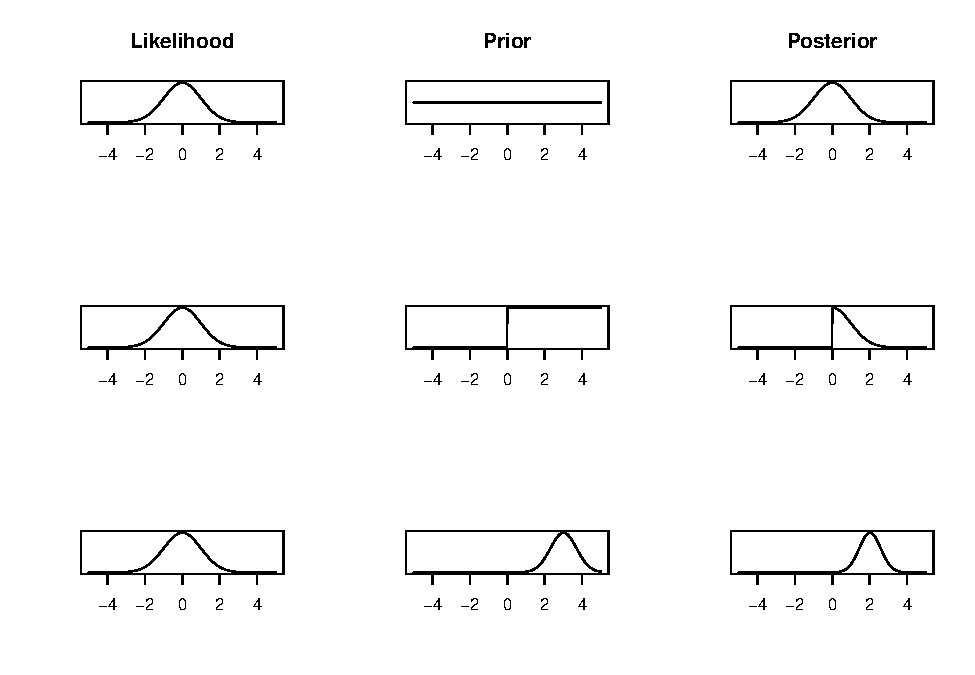
\includegraphics{_main_files/figure-latex/unnamed-chunk-6-1.pdf}

\begin{enumerate}
\def\labelenumi{\arabic{enumi}.}
\item
  The posterior distribution is proportional to the likelihood function. The prior distribution closely matches frequentist inference. Both the MLE and posterior mean are 0.
\item
  We get a lopsided posterior distribution, that is proportional to the likelihood function for positive values of \(\theta\), but is 0 for negative values of \(\theta\).
\end{enumerate}

3.We get some sort of average of the likelihood fucntion and the prior distribution. Had we collected more data, the posterior distirbution would have been weighted toward the information from the likelihood function more.
\end{example}

\hypertarget{programming-in-r}{%
\chapter{Programming in R}\label{programming-in-r}}

\hypertarget{bayesian-inference}{%
\chapter{Bayesian inference}\label{bayesian-inference}}

Whereas Chapter 1 dealt with the fundamentals of Bayesian inference and definitions, Chapter 2 is much more practical. We're going to be deriving posterior distributions and proving when it does and doesn't work.

\hypertarget{the-binomial-distirbution}{%
\section{The Binomial distirbution}\label{the-binomial-distirbution}}

The first example we're going to go through is with the binomial distribution.

\begin{example}
\protect\hypertarget{exm:binom}{}\label{exm:binom}A technician in a crisp factory wants to test the reliability of a production line. She collects a random sample of 200 crisp packets from line 1. She finds three packets weigh either too much or too little and must be rejected. She uses a Bayesian method to estimate the probability a crisp packet is the incorrect weight. She begins by denoting the weight of the 200 crisp packets \(\boldsymbol{y} = \{y_1, \ldots, y_{200}\}\) and the probability a crisp packet is the incorrect weight by \(\theta\). By Bayes' theorem
\[
p(\theta \mid \boldsymbol{y}) \propto p(\boldsymbol{y}\mid \theta) p(\theta)
\]

\textbf{Likelihood function} \(p(\boldsymbol{y}\mid \theta)\). We observe a 200 trials each with a probability of success or failure. The binomial distribution seems the most suitable way of modelling this. Therefore
\[
p(\boldsymbol{y}\mid \theta) = \begin{pmatrix} 200 \\ 3 \end{pmatrix} \theta^3(1-\theta)^{197}
\]
We are going to ignore one questionable assumption here that the observations are independent. That is a crisp packet being the wrong weight, doesn't affect the weight of the next crisp packet to be produced.

\textbf{Prior distribution} \(p(\theta)\). We now need to describe our prior beliefs about \(\theta\). We have no reason to suggest \(\theta\) takes any specific value, so we use a uniform prior distribution \(\theta \sim U[0, 1]\), where \(p(\theta) = 1\) for \(\theta \in [0, 1]\).

\textbf{Posterior distribution} \(p(\theta \mid \boldsymbol{y})\). We can now derive the posterior distribution up to proportionality
\[
p(\theta \mid \boldsymbol{y}) \propto \theta^3(1-\theta)^{197}. 
\]
This functional dependence on p identifies the \(p(\theta \mid \boldsymbol{y})\) as a Beta distribution. The PDF for the beta distribution with shape parameters \(\alpha\) and \(\beta\) is
\[
p(x \mid \alpha, \beta) = \frac{\Gamma(\alpha + \beta)}{\Gamma(\alpha)\Gamma(\beta)}x^{\alpha - 1}(1-x)^{\beta - 1}. 
\]
The posterior distribution is therefore \(\theta \mid \boldsymbol{y} \sim \textrm{Beta}(4, 198)\).
\end{example}

\hypertarget{reporting-conclsuions-from-bayesian-inference}{%
\section{Reporting conclsuions from Bayesian inference}\label{reporting-conclsuions-from-bayesian-inference}}

In th previous example, we derived the posterior distribution \(\theta \mid \boldsymbol{y} \sim \textrm{Beta}(4, 198)\). But often, we want to share more descriptive information about our beliefs given the observed data. In this example, the posterior mean given the data is \(\frac{4}{198} = \frac{2}{99}\). That is to say given the data, we expect that for every 99 packets of crisps produced, two will be the incorrect weight. The posterior mode for \(\theta\) is \(\frac{3}{200}\) or 1.5\%.

It is important to share the uncertainty about out beliefs. In a frequentist framework, this would be via a confidence interval. The Bayesian analogues is a credible interval.

\begin{definition}
A \textbf{credible interval} is a central interval of posterior probability which corresponds, in the case of a 100\((1-\alpha)\)\% interval, to the range of values that capture 100\((1-\alpha)\)\% of the posterior probability.
\end{definition}

\begin{example}
The 95\% credible interval for the Binomial example is given by

\begin{Shaded}
\begin{Highlighting}[]
\NormalTok{cred.int}\FloatTok{.95} \OtherTok{\textless{}{-}} \FunctionTok{qbeta}\NormalTok{(}\FunctionTok{c}\NormalTok{(}\FloatTok{0.025}\NormalTok{, }\FloatTok{0.975}\NormalTok{), }\DecValTok{4}\NormalTok{, }\DecValTok{198}\NormalTok{)}
\FunctionTok{round}\NormalTok{(cred.int}\FloatTok{.95}\NormalTok{, }\DecValTok{3}\NormalTok{)}
\end{Highlighting}
\end{Shaded}

\begin{verbatim}
## [1] 0.005 0.043
\end{verbatim}

This says that we believe there is a 95\% chance that the probability of a crisp packet being the incorrect weight lies between 0.005 and 0.043. This is a much more intuitive definition to the confidence interval, which says if we ran the experiment an infinite number of times and computed an infinite number of confidence intervals, 95\% of them would contain the true value of \(\theta\).
\end{example}

\hypertarget{the-exponential-distribution}{%
\section{The Exponential distribution}\label{the-exponential-distribution}}

\begin{example}

An insurance company want to estimate the time until a claim is made on a specific policy. They describe the rate at which claims come in by \(\lambda\). The company provides a sample of 10 months at which a claim was made \(\boldsymbol{y} = \{14, 10, 6, 7, 13, 9, 12, 7, 9, 8\}\). By Bayes' theorem, the posterior distribution for \(\lambda\) is
\[
p(\lambda \mid \boldsymbol{y}) \propto p(\lambda \mid \boldsymbol{y}) p(\lambda)
\]

\textbf{Likelihood function} \(p(\lambda \mid \boldsymbol{y})\). The exponential distribution is a good way of modelling lifetimes or the length of time until an event happens. Assuming all the claims are independent, the likelihood function is given by
\begin{align*}
p(\boldsymbol{y} \mid \lambda) &= \prod_{i=1}^{10} \lambda e^{-\lambda y_i} \\
& = \lambda^{10}e^{-\lambda \sum_{i=1}^{10} y_i} \\
& = \lambda^{10} e^{-95\lambda}
\end{align*}

\textbf{Prior distribution} \(p(\lambda)\). As we are modelling a rate parameter, we know it must be positive and continuous. We decide to use an exponential prior distribution for \(\lambda\), but leave the choice of the rate parameter up to the insurance professionals at the insurance company. The prior distribution is given by \(p(\lambda) \sim \textrm{Exp}(\chi).\)

\textbf{Posterior distribution} \(p(\lambda \mid \boldsymbol{y})\). We now have all the ingredients to derive the posterior distribution. It is given by
\begin{align*}
p(\lambda \mid \boldsymbol{y}) &\propto \lambda^{10} e^{-95\lambda} \times \lambda e^{-\chi\lambda} \\
& \propto \lambda^{11}e^{-(95 + \chi)\lambda}
\end{align*}
The functional form tells us that the posterior distribution is a Gamma distribution. The PDF of a gamma random variable with shape \(\alpha\) and rate \(\beta\) is
\[
p(x \mid \alpha, \beta) = \frac{\alpha^\beta}{\Gamma(\alpha)}x^{\alpha-1}e^{-\beta x}.
\]
The distribution of the rate of the claims given the observed data is \(\lambda \mid \boldsymbol{y} \sim \textrm{Gamma}(10, 95 + \chi)\).

The posterior mean months until a claim is \(\frac{10}{95 + \chi}\). We can see the effect of the choice of rate parameter in this mean. Small values of \(\chi\) yield vague prior distribution, which plays a minimal role in the posterior distribution. Large values of \(\chi\) result in prior distributions that contribute a lot to the posterior distribution. The plots below show the prior and posterior distibrutions for \(\chi = 0.01\) and \(\chi = 50\).

\begin{Shaded}
\begin{Highlighting}[]
\NormalTok{plot.distributions }\OtherTok{\textless{}{-}} \ControlFlowTok{function}\NormalTok{(chi)\{}
  \CommentTok{\#evaluate at selected values of theta}
\NormalTok{  theta }\OtherTok{\textless{}{-}} \FunctionTok{seq}\NormalTok{(}\FloatTok{0.001}\NormalTok{, }\FloatTok{0.3}\NormalTok{, }\FloatTok{0.001}\NormalTok{) }
  
  \CommentTok{\#evaluate prior desnity}
\NormalTok{  prior }\OtherTok{\textless{}{-}} \FunctionTok{dexp}\NormalTok{(theta, }\AttributeTok{rate =}\NormalTok{ chi)}
  
  \CommentTok{\#evaluate posterior density}
\NormalTok{  posterior }\OtherTok{\textless{}{-}} \FunctionTok{dgamma}\NormalTok{(theta, }\AttributeTok{shape =} \DecValTok{10}\NormalTok{, }\AttributeTok{rate =} \DecValTok{95} \SpecialCharTok{+}\NormalTok{ chi)}
  
  
  \CommentTok{\#plot}
  \FunctionTok{plot}\NormalTok{(theta, posterior, }\AttributeTok{type=} \StringTok{\textquotesingle{}l\textquotesingle{}}\NormalTok{, }
       \AttributeTok{ylim =} \FunctionTok{c}\NormalTok{(}\DecValTok{0}\NormalTok{, }\DecValTok{50}\NormalTok{), }\AttributeTok{xlab =} \FunctionTok{expression}\NormalTok{(theta), }\AttributeTok{ylab =} \StringTok{"density"}\NormalTok{)}
  \FunctionTok{lines}\NormalTok{(theta, prior, }\AttributeTok{lty =} \DecValTok{2}\NormalTok{)}
  \FunctionTok{legend}\NormalTok{(}\StringTok{\textquotesingle{}topright\textquotesingle{}}\NormalTok{, }\AttributeTok{lty =} \FunctionTok{c}\NormalTok{(}\DecValTok{1}\NormalTok{, }\DecValTok{2}\NormalTok{), }\AttributeTok{legend =} \FunctionTok{c}\NormalTok{(}\StringTok{"Posterior"}\NormalTok{, }\StringTok{"Prior"}\NormalTok{),  }
         \AttributeTok{bty =} \StringTok{"n"}\NormalTok{)}
\NormalTok{\}}

\FunctionTok{plot.distributions}\NormalTok{(}\FloatTok{0.01}\NormalTok{)}
\end{Highlighting}
\end{Shaded}

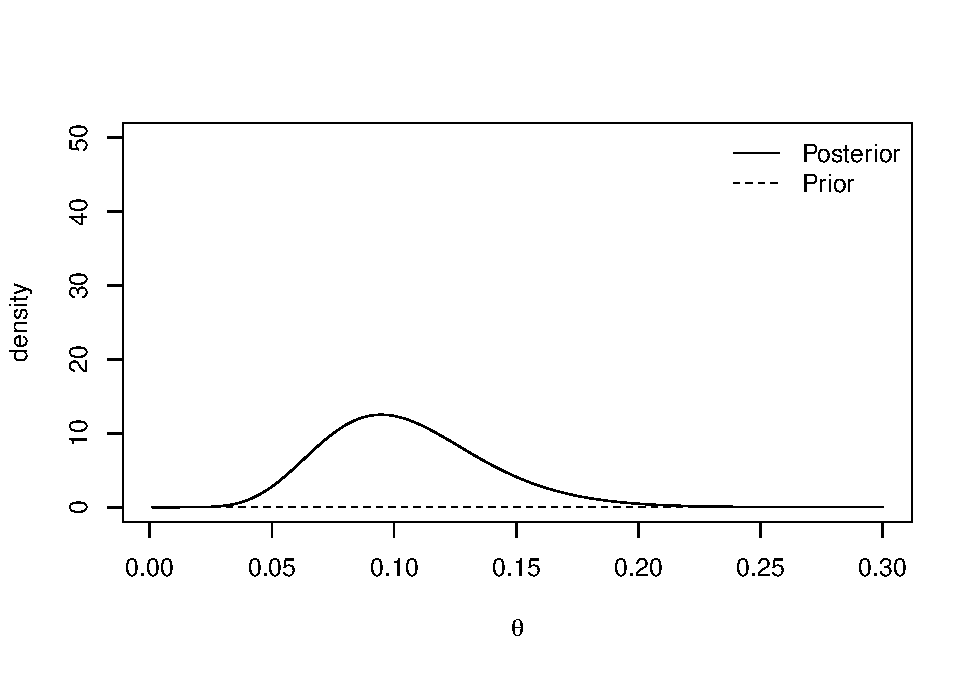
\includegraphics{_main_files/figure-latex/unnamed-chunk-8-1.pdf}

\begin{Shaded}
\begin{Highlighting}[]
\FunctionTok{plot.distributions}\NormalTok{(}\DecValTok{50}\NormalTok{)}
\end{Highlighting}
\end{Shaded}

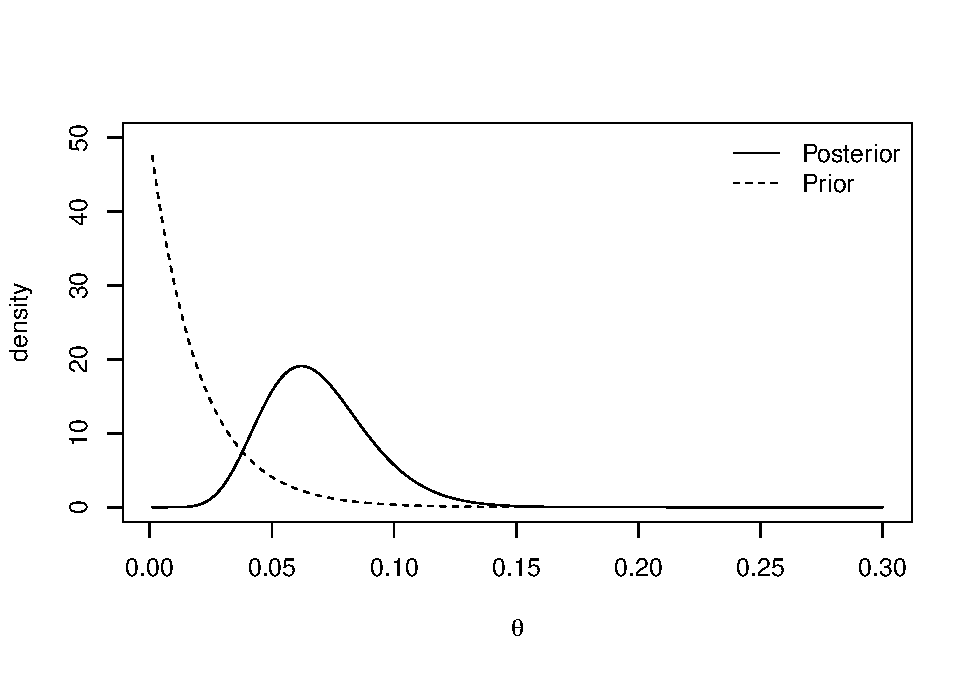
\includegraphics{_main_files/figure-latex/unnamed-chunk-8-2.pdf}

The insurance managers recommend that because this is a new premium, a vague prior distribution be used and \(\chi = 0.01\). The posterior mean is \(\frac{10}{95.01} \approx 0.105\) and the 95\% credible interval is

\begin{Shaded}
\begin{Highlighting}[]
\FunctionTok{round}\NormalTok{(}\FunctionTok{qgamma}\NormalTok{(}\FunctionTok{c}\NormalTok{(}\FloatTok{0.025}\NormalTok{, }\FloatTok{0.975}\NormalTok{), }\DecValTok{10}\NormalTok{, }\FloatTok{95.01}\NormalTok{), }\DecValTok{3}\NormalTok{)}
\end{Highlighting}
\end{Shaded}

\begin{verbatim}
## [1] 0.05 0.18
\end{verbatim}

\end{example}

\hypertarget{predicition}{%
\section{Predicition}\label{predicition}}

In many cases, although we are interested in estimating the model parameters, what we're really interested in is predicting new values, whose distribution is determined by the model parameters.

\begin{definition}
Suppose we observe some data \(\boldsymbol{y}\) and derive the posterior distribution \(\pi(\theta \mid \boldsymbol{y})\). The quantity we are interested in is some future observation \(z\), we would like to the distribution of \(z\) given the observed data \(\boldsymbol{y}\), \(p(z \mid \boldsymbol{y})\). This distribution, known as the \textbf{posterior predictive distribution} of \(z\), must be exhibited as a mixture distribution over the possible values of \(\theta\). We must write
\[
p(z \mid \boldsymbol{y}) = \int \pi(z \mid \theta) \pi(\theta \mid \boldsymbol{y})\, d\theta.
\]
\end{definition}

\begin{example}

Students have to submit coursework for a particular statistical modules. However, each semester a number of students miss the deadline and hand in their coursework late. Last year, three out of 20 students handed their coursework in late. This year, the course has thirty students in. How many students can we expect to hand in their coursework late?

We can model the number of students handing in late \(X\), using a Binomial distribution, \(Y \sim \textrm{Bin}(n, \theta)\). As in Example \ref{exm:binom}, we assign a uniform prior distribution to \(\theta \sim U[0, 1]\). Given then observed data, we can derive \(\theta \mid \boldsymbol{y} \sim Beta(4, 28)\) (See problem sheets for derivation).

Now we can derive the posterior predictive distribution of \(Z\), the number of students who hand in late. We model \(Z\) using a Binomial distribution, \(Z \sim \textrm{Bin}(30, \theta)\). The distribution of \(Z\) given the observed data is

\begin{align*}
p(z \mid \boldsymbol{y}) &= \int_0^1 \pi(z \mid \theta) \pi(\theta \mid \boldsymbol{y})\, d\theta \\
& = \int_0^1 \begin{pmatrix} 30 \\ z \end{pmatrix} \theta^z (1-\theta)^{30 - z} \frac{\Gamma(32)}{\Gamma(4)\Gamma(28)}\theta^{3}(1-\theta)^{27}\, d\theta \\
 & = \begin{pmatrix} 30 \\ z \end{pmatrix}\frac{\Gamma(32)}{\Gamma(4)\Gamma(28)}\int_0^1 \theta^{z + 3}(1-\theta)^{57 - z}\, d\theta \\
\end{align*}
This integral is difficult to evaluate immediately. But by multiplying (and dividing outside the integral) by a constant, we can turn it into the density function of a Beta\((5 + z, 58 - z)\) random variable. This integrates to 1.

\begin{align*}
p(z \mid \boldsymbol{y})  & = \begin{pmatrix} 30 \\ z \end{pmatrix}\frac{\Gamma(32)}{\Gamma(4)\Gamma(28)}\frac{\Gamma(z+4)\Gamma(58-z)}{\Gamma(62)}\int_0^1 \frac{\Gamma(62)}{\Gamma(z+4)\Gamma(58-z)}\theta^{z + 3}(1-\theta)^{57 - z}\, d\theta \\ 
& = \begin{pmatrix} 30 \\ z \end{pmatrix}\frac{\Gamma(32)\Gamma(z+4)\Gamma(58-z)}{\Gamma(4)\Gamma(28)\Gamma(62)} \quad \textrm{for } 0 \leq z \leq 30.
\end{align*}

This code implements the distribution

\begin{Shaded}
\begin{Highlighting}[]
\NormalTok{beta.binom.posterior.predictive.distribution }\OtherTok{\textless{}{-}} \ControlFlowTok{function}\NormalTok{(z)\{}
  
  
\NormalTok{  numerator }\OtherTok{\textless{}{-}} \FunctionTok{gamma}\NormalTok{(}\DecValTok{32}\NormalTok{)}\SpecialCharTok{*}\FunctionTok{gamma}\NormalTok{(z }\SpecialCharTok{+} \DecValTok{4}\NormalTok{)}\SpecialCharTok{*}\FunctionTok{gamma}\NormalTok{(}\DecValTok{58}\SpecialCharTok{{-}}\NormalTok{z)}
\NormalTok{  denominator }\OtherTok{\textless{}{-}} \FunctionTok{gamma}\NormalTok{(}\DecValTok{4}\NormalTok{)}\SpecialCharTok{*}\FunctionTok{gamma}\NormalTok{(}\DecValTok{28}\NormalTok{)}\SpecialCharTok{*}\FunctionTok{gamma}\NormalTok{(}\DecValTok{62}\NormalTok{)}
  
\NormalTok{  output }\OtherTok{\textless{}{-}} \FunctionTok{choose}\NormalTok{(}\DecValTok{30}\NormalTok{, z)}\SpecialCharTok{*}\NormalTok{numerator}\SpecialCharTok{/}\NormalTok{denominator}
  \FunctionTok{return}\NormalTok{(output)}
  
\NormalTok{\}}
\end{Highlighting}
\end{Shaded}

We can check it's correct, by seeing if it sums to one

\begin{Shaded}
\begin{Highlighting}[]
\NormalTok{z }\OtherTok{\textless{}{-}} \DecValTok{0}\SpecialCharTok{:}\DecValTok{30}
\NormalTok{ppd }\OtherTok{\textless{}{-}} \FunctionTok{beta.binom.posterior.predictive.distribution}\NormalTok{(z)}
\FunctionTok{sum}\NormalTok{(ppd)}
\end{Highlighting}
\end{Shaded}

\begin{verbatim}
## [1] 1
\end{verbatim}

\begin{Shaded}
\begin{Highlighting}[]
\FunctionTok{plot}\NormalTok{(z, ppd, }\AttributeTok{xlab =} \StringTok{"z"}\NormalTok{, }\AttributeTok{ylab =} \FunctionTok{expression}\NormalTok{(}\FunctionTok{p}\NormalTok{(z }\SpecialCharTok{|}\NormalTok{ theta)))}
\end{Highlighting}
\end{Shaded}

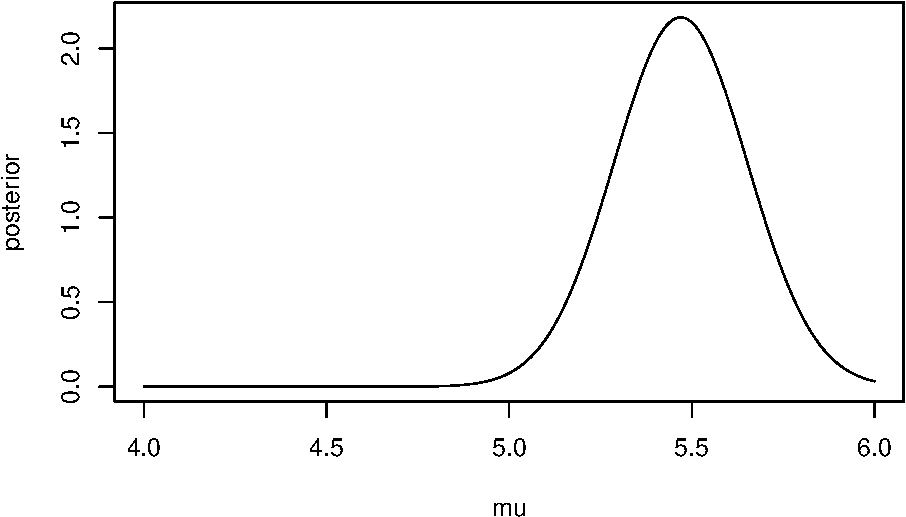
\includegraphics{_main_files/figure-latex/unnamed-chunk-11-1.pdf}
The expected number of students who hand in late is 3.75 and there's a 95\% chance that up to 8 hand in late.

\begin{Shaded}
\begin{Highlighting}[]
\NormalTok{z}\SpecialCharTok{\%*\%}\NormalTok{ppd }\CommentTok{\#expectation}
\end{Highlighting}
\end{Shaded}

\begin{verbatim}
##      [,1]
## [1,] 3.75
\end{verbatim}

\begin{Shaded}
\begin{Highlighting}[]
\FunctionTok{cbind}\NormalTok{(z, }\FunctionTok{cumsum}\NormalTok{(ppd)) }\CommentTok{\#CDF}
\end{Highlighting}
\end{Shaded}

\begin{verbatim}
##        z           
##  [1,]  0 0.06029453
##  [2,]  1 0.18723037
##  [3,]  2 0.35156696
##  [4,]  3 0.51889148
##  [5,]  4 0.66530044
##  [6,]  5 0.78021765
##  [7,]  6 0.86309065
##  [8,]  7 0.91880359
##  [9,]  8 0.95404202
## [10,]  9 0.97513714
## [11,] 10 0.98713498
## [12,] 11 0.99363285
## [13,] 12 0.99698773
## [14,] 13 0.99863936
## [15,] 14 0.99941423
## [16,] 15 0.99976022
## [17,] 16 0.99990696
## [18,] 17 0.99996591
## [19,] 18 0.99998826
## [20,] 19 0.99999622
## [21,] 20 0.99999887
## [22,] 21 0.99999969
## [23,] 22 0.99999992
## [24,] 23 0.99999998
## [25,] 24 1.00000000
## [26,] 25 1.00000000
## [27,] 26 1.00000000
## [28,] 27 1.00000000
## [29,] 28 1.00000000
## [30,] 29 1.00000000
## [31,] 30 1.00000000
\end{verbatim}

\end{example}

\hypertarget{non-informative-prior-distibrutions}{%
\section{Non-informative prior distibrutions}\label{non-informative-prior-distibrutions}}

We have seen in a few examples how the choice of prior distribution can affect that posterior distributions and the resulting conclusions. As the choice of prior distribution is subjective, it is the main criticism of Bayesian inference. A possible way around this is to use a prior distribution that reflects a lack of information about \(\theta\).

\begin{definition}
A \textbf{non-informative prior distribution} is a prior distribution that places equal weight on the every possible value of \(\theta\).
\end{definition}

\begin{example}
In Example \ref{exm:binom}, we assigned a uniform prior distribution to the parameter \(\theta\).
\end{example}

\begin{theorem}[Jeffrey]
Given some observed data \(\boldsymbol{y} = \{y_1, \ldots, y_N\}\), an invariant prior distribution is
\[
p(\theta) \propto \sqrt{I_\theta(\boldsymbol{y})},
\]
where \(I_\theta(\boldsymbol{y})\) is the Fisher information for \(\theta\) contained in \(\boldsymbol{y}\).
\end{theorem}

Jeffrey argues that if there are two ways of parameterising a model, e.g.~via \(\theta\) and \(\psi\), then the priors on these parameters should be equivalent. In other words, the prior distribution should be invariant under sensible (one-to-one) transformations.

\begin{proof}
Recall that the distribution of \(\psi = h(\theta)\), for some one-to-one function \(h\), is invariant to the distribution of \(\theta\) if
\[
p(\psi) = p(\theta) \left|\frac{d\theta}{d\psi}\right|.
\]

Transforming the Fisher information for \(\psi\) shows
\begin{align*}
I_\psi(\boldsymbol{y}) &= - \mathbb{E}\left(\frac{d^2\log p(\boldsymbol{y} \mid \psi)}{d\psi^2}\right) \\
& = \mathbb{E}\left(\frac{d^2 \log p(\boldsymbol{y} \mid \theta = h^{-1}(\psi))}{d\theta^2}\right) \left(\frac{d\theta}{d\psi}\right)^2 \\
& = I_\theta(\boldsymbol{y})\left(\frac{d\theta}{d\psi}\right)^2 .
\end{align*}
Thus \(\sqrt{I_\psi(\boldsymbol{y})} = \sqrt{I_\theta(\boldsymbol{y})} \left|\frac{d\theta}{d\psi}\right|\) and \(\sqrt{I_\psi(\boldsymbol{y})}\) and \(\sqrt{I_\theta(\boldsymbol{y})}\) are invariant prior distributions.
\end{proof}

\begin{example}
In example \ref{exm:binom}, we modelled the number of crisps that were the incorrect weight by \(\theta \sim \textrm{Bin}(n, \theta)\). To construct Jeffrey's prior distribution for \(\theta\), we must first derive the Fisher's information matrix.\\
\begin{align*}
&p(y \mid \theta) = \begin{pmatrix} n \\ y \end{pmatrix} \theta^y (1-\theta)^{n-y}\\ 
\implies &\log p(y \mid \theta) = \log \begin{pmatrix} n \\ y \end{pmatrix} + y \log\theta + (n-y)\log(1-\theta) \\
\implies &\frac{\partial \log p(y \mid \theta)}{\partial \theta} = \frac{y}{\theta} - \frac{n-y}{1-\theta} \\
\implies &\frac{\partial^2 \log p(y \mid \theta)}{\partial \theta^2} = -\frac{y}{\theta^2} + \frac{n-y}{(1-\theta)^2} \\
\implies &\mathbb{E}\left(\frac{\partial \log p(y \mid \theta)}{\partial \theta}\right) = -\frac{\mathbb{E}(y)}{\theta^2} + \frac{n-\mathbb{E}(y)}{(1-\theta)^2}\\ 
\implies &\mathbb{E}\left(\frac{\partial \log p(y \mid \theta)}{\partial \theta}\right) = -\frac{n\theta}{\theta^2} + \frac{n-n\theta}{(1-\theta)^2}\\ 
\implies &\mathbb{E}\left(\frac{\partial \log p(y \mid \theta)}{\partial \theta}\right) = -\frac{n}{\theta} + \frac{n}{1-\theta}\\
\implies &\mathbb{E}\left(\frac{\partial \log p(y \mid \theta)}{\partial \theta}\right) = -\frac{n}{\theta(1-\theta)} \\
\implies &I_\theta(y) \propto \frac{1}{\theta(1-\theta)}.
\end{align*}
\$
Hence Jeffrey's prior is \(p(\theta) \propto \theta^{-\frac{1}{2}}(1-\theta)^{-\frac{1}{2}}\). This functional dependency on \(\theta\) shows that \(\theta \sim \textrm{Beta}(\frac{1}{2}, \frac{1}{2})\).
\end{example}

\hypertarget{bernstein-von-mises-theorem}{%
\section{Bernstein-von-Mises Theorem}\label{bernstein-von-mises-theorem}}

So far, we have considered Bayesian methods in contrast to frequentist ones. The Bernstein-von-Mises theorem is a key theorem linking the two inference methods.

\begin{theorem}[Bernstein-von-Mises]
For a well-specified model \(p(\boldsymbol{y} \mid \theta)\) with a fixed number of parameters, and for a smooth prior distribution \(p(\theta)\) that is non-zero around the MLE \(\hat{\theta}\), then
\[
\left|\left| p(\theta \mid \boldsymbol{y}) - N\left(\hat{\theta}, \frac{I(\hat{\theta})^{-1}}{n}\right) \right|\right|_{TV} \rightarrow 0,
\]
where \(||p - q||_{TV}\) is the total variation distance between distributions \(p\) and \(q\):
\[
||p - q||_{TV} = \frac{1}{2}\int|p(x) - q(x)|\,dx.
\]
\end{theorem}

The Berstein-von-Mises theorem says that as the number of data points approaches infinity, the posterior distribution tends to a Normal distribution centered around the MLE and variance dependent on the Fisher information.

\hypertarget{sampling}{%
\chapter{Sampling}\label{sampling}}

\hypertarget{uniform-random-numbers}{%
\section{Uniform random numbers}\label{uniform-random-numbers}}

What we won't be doing in this module is generating true uniform random numbers. This is incredibly difficult and usually requires lots of expensive hardware. This is because computers aren't good at being random, they require algorithmic instructions. True random number generation often uses physical methods, such as the radioactive decay of atoms, or atmospheric noise.

Throughout this module, we will be using R's built in random number generation. This is a pseudo random number generator, that has excellent random properties, but will eventually repeat. A basic random number generation method is sampling from a uniform distribution on the unit interval

\begin{Shaded}
\begin{Highlighting}[]
\FunctionTok{runif}\NormalTok{(}\DecValTok{1}\NormalTok{, }\DecValTok{0}\NormalTok{, }\DecValTok{1}\NormalTok{)}
\end{Highlighting}
\end{Shaded}

\begin{verbatim}
## [1] 0.08712486
\end{verbatim}

\hypertarget{inverse-transform-sampling}{%
\section{Inverse transform sampling}\label{inverse-transform-sampling}}

Suppose we want to sample from a non-uniform one-dimensional distribution. The inverse transform theorem allows us to do this using the distribution's inverse function.

\begin{definition}
The \textbf{inverse function} of a distribution \(F\), denoted \(F^{-1}\), is defined for all \(u \in (0, 1)\) by
\[
F^{-1}(u) = \inf\{x \in\mathbb{R} : F(x) > u\}.
\]
\end{definition}

\begin{theorem}
Let \(F :\mathbb{R} \rightarrow [0, 1]\), \(U \sim U[0, 1]\) and \(Y = F^{-1}(U)\). Then \(Y\) has distribution \(F\).
\end{theorem}

\begin{proof}
We have
\[
p(Y \leq a) = p(F^{-1}(U) \leq a) = p(\inf\{x \in\mathbb{R} : F(x) > u\} \leq a). 
\]
Since \(\inf\{x \in\mathbb{R} : F(x) > u\} \leq a\) can only hold if \(F(a) \geq U\), we have
\[
p(Y \leq a)  = p(F(a)\geq U)
\]
As \(U \sim U[0, 1]\), we have \(p(F(a)\geq U) = F(a)\).
\end{proof}

This theorem says that if we have a random variable \(U \sim U[0, 1]\) and we want to get \(Y \sim F\), then we can use \(F^{-1}(U)\). Viewing this theorem graphically can provide a much more intuitive understanding.

\begin{example}
We would like to sample from an exponential distribution with rate 0.5. The likelihood function is given by
\[
p(y \mid \lambda = 0.5) = 0.5e^{0.5y}.
\]
The distribution function can be derived by
\begin{align*}
F(y \mid \lambda = 0.5) &= \int_0^y 0.5e^{0.5t}\,dt \\
& =  1 - e^{0.5y}.
\end{align*}
Finally, the inverse function is given by
\[
F^{-1}(y \mid \lambda = 0.5) = -2\log(1-y).  
\]
Therefore, if \(U \sim U[0, 1]\), \(-2\log(1-U) \sim \hbox{Exp}(0.5)\).

The R code below generates a plot to show this. We can plot the CDF for most one parameter distributions straightforwardly. We can think of this theorem as allowing us to sample a point on the y-axis and then computing the quantile this corresponds to.

\begin{Shaded}
\begin{Highlighting}[]
\FunctionTok{set.seed}\NormalTok{(}\DecValTok{12345}\NormalTok{) }\CommentTok{\# to reproduce}
\NormalTok{y }\OtherTok{\textless{}{-}} \FunctionTok{seq}\NormalTok{(}\DecValTok{0}\NormalTok{, }\DecValTok{10}\NormalTok{, }\FloatTok{0.01}\NormalTok{) }\CommentTok{\#Show on the interval [0, 5]}
\NormalTok{f }\OtherTok{\textless{}{-}} \DecValTok{1} \SpecialCharTok{{-}} \FunctionTok{exp}\NormalTok{(}\SpecialCharTok{{-}}\FloatTok{0.5}\SpecialCharTok{*}\NormalTok{y)    }\CommentTok{\#Construct the cumulative density function (CDF)}
\FunctionTok{plot}\NormalTok{(y, f, }\AttributeTok{type =}\StringTok{\textquotesingle{}l\textquotesingle{}}\NormalTok{, }\AttributeTok{xlab =} \StringTok{"y"}\NormalTok{, }\AttributeTok{ylab=} \StringTok{"CDF"}\NormalTok{)}

\CommentTok{\#Sample u}
\NormalTok{u }\OtherTok{\textless{}{-}} \FunctionTok{runif}\NormalTok{(}\DecValTok{1}\NormalTok{)}

\CommentTok{\#Get the corresponding y value}
\NormalTok{f.inv }\OtherTok{\textless{}{-}} \SpecialCharTok{{-}}\DecValTok{2}\SpecialCharTok{*}\FunctionTok{log}\NormalTok{(}\DecValTok{1}\SpecialCharTok{{-}}\NormalTok{u)}

\CommentTok{\#plot }
\FunctionTok{segments}\NormalTok{(}\AttributeTok{x0 =} \DecValTok{0}\NormalTok{, }\AttributeTok{y0 =}\NormalTok{ u, }\AttributeTok{x1 =}\NormalTok{ f.inv, }\AttributeTok{y1 =}\NormalTok{ u, }\AttributeTok{lty =} \DecValTok{2}\NormalTok{)}
\FunctionTok{segments}\NormalTok{(}\AttributeTok{x0 =}\NormalTok{ f.inv, }\AttributeTok{y0 =} \DecValTok{0}\NormalTok{, }\AttributeTok{x1 =}\NormalTok{ f.inv, }\AttributeTok{y1 =}\NormalTok{ u, }\AttributeTok{lty =} \DecValTok{2}\NormalTok{)}
\end{Highlighting}
\end{Shaded}

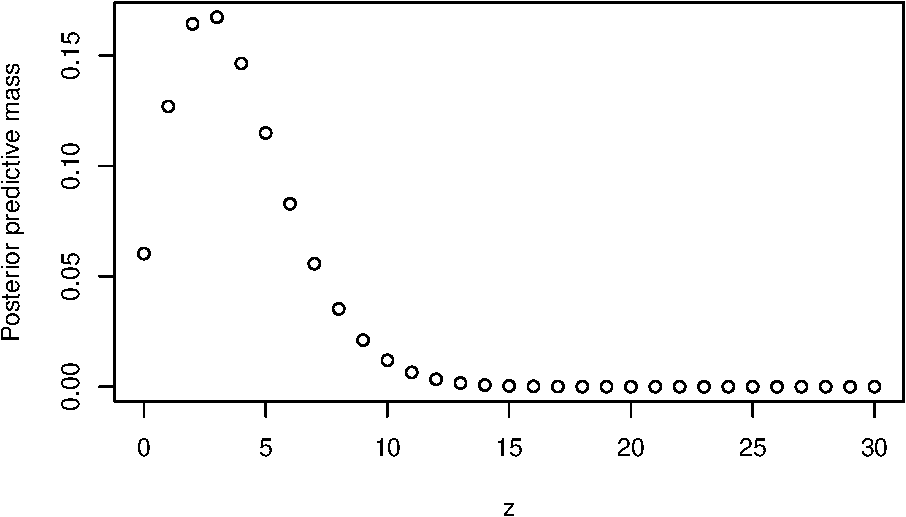
\includegraphics{_main_files/figure-latex/unnamed-chunk-14-1.pdf}
\end{example}

\hypertarget{rejection-sampling}{%
\section{Rejection sampling}\label{rejection-sampling}}

A more common method to draw samples from a distribution is called rejection sampling. It works generating numbers from some distribution we can work with and then evaluating if the random numbers qualify for the distribution we are interested in.

\begin{example}
A non-distributional example of this is estimating \(\pi\). We first generate 1,000 points on the unit square \((x, y) \in \{[0, 1] \times [0, 1]\}\). We evaluate if each point falls within the unit circle, i.e.~\(x^2 + y^2 < 1\). The propotion of the points that meet this criteria is approximately \(\frac{pi}{4}\).

\begin{Shaded}
\begin{Highlighting}[]
\CommentTok{\#Generate random coordinates}
\NormalTok{N }\OtherTok{\textless{}{-}} \DecValTok{1000}
\NormalTok{x }\OtherTok{\textless{}{-}} \FunctionTok{runif}\NormalTok{(N)}
\NormalTok{y }\OtherTok{\textless{}{-}} \FunctionTok{runif}\NormalTok{(N)}

\CommentTok{\#Compute how many are in the circle}
\NormalTok{in.circle }\OtherTok{\textless{}{-}} \FunctionTok{ifelse}\NormalTok{(x}\SpecialCharTok{\^{}}\DecValTok{2} \SpecialCharTok{+}\NormalTok{ y}\SpecialCharTok{\^{}}\DecValTok{2} \SpecialCharTok{\textless{}} \DecValTok{1}\NormalTok{, }\DecValTok{1}\NormalTok{, }\DecValTok{0}\NormalTok{)}

\CommentTok{\#Aproximate pi}
\DecValTok{4}\SpecialCharTok{*}\FunctionTok{sum}\NormalTok{(in.circle)}\SpecialCharTok{/}\NormalTok{N}
\end{Highlighting}
\end{Shaded}

\begin{verbatim}
## [1] 3.104
\end{verbatim}

\begin{Shaded}
\begin{Highlighting}[]
\NormalTok{(}\DecValTok{4}\SpecialCharTok{*}\FunctionTok{sum}\NormalTok{(in.circle)}\SpecialCharTok{/}\NormalTok{N }\SpecialCharTok{{-}}\NormalTok{ pi)}\SpecialCharTok{/}\NormalTok{pi}\SpecialCharTok{*}\DecValTok{100} \CommentTok{\#\%relative error}
\end{Highlighting}
\end{Shaded}

\begin{verbatim}
## [1] -1.196611
\end{verbatim}

\begin{Shaded}
\begin{Highlighting}[]
\CommentTok{\#A nice plot}
\FunctionTok{plot}\NormalTok{(x, y, }\AttributeTok{pch =} \DecValTok{4}\NormalTok{, }\AttributeTok{col =} \FunctionTok{rgb}\NormalTok{(}\DecValTok{0}\NormalTok{, }\DecValTok{0}\NormalTok{, }\DecValTok{0}\NormalTok{, }\FloatTok{0.1}\NormalTok{))}
\NormalTok{theta }\OtherTok{\textless{}{-}} \FunctionTok{seq}\NormalTok{(}\DecValTok{0}\NormalTok{, pi}\SpecialCharTok{/}\DecValTok{2}\NormalTok{, }\FloatTok{0.01}\NormalTok{)}
\FunctionTok{lines}\NormalTok{(}\AttributeTok{x =} \FunctionTok{cos}\NormalTok{(theta), }\AttributeTok{y =} \FunctionTok{sin}\NormalTok{(theta))}
\FunctionTok{points}\NormalTok{(x[in.circle }\SpecialCharTok{==} \DecValTok{1}\NormalTok{], y[in.circle }\SpecialCharTok{==} \DecValTok{1}\NormalTok{], }\AttributeTok{pch =} \DecValTok{4}\NormalTok{, }\AttributeTok{col =} \FunctionTok{rgb}\NormalTok{(}\DecValTok{1}\NormalTok{, }\DecValTok{0}\NormalTok{, }\DecValTok{0}\NormalTok{, }\FloatTok{0.1}\NormalTok{))}
\end{Highlighting}
\end{Shaded}

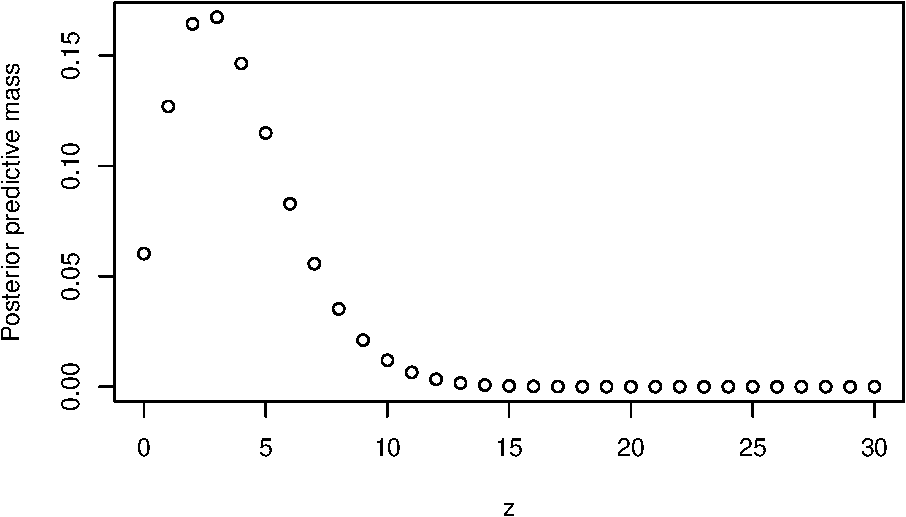
\includegraphics{_main_files/figure-latex/unnamed-chunk-15-1.pdf}
\end{example}

\hypertarget{monte-carlo}{%
\section{Monte Carlo}\label{monte-carlo}}

\hypertarget{markov-chain-monte-carlo}{%
\section{Markov Chain Monte Carlo}\label{markov-chain-monte-carlo}}

\hypertarget{advanced-computation}{%
\chapter{Advanced computation}\label{advanced-computation}}

  \bibliography{book.bib,packages.bib}

\end{document}
